% \documentclass[14pt,twoside,open=right]{scrreprt}
\documentclass[14pt]{scrreprt}
\usepackage[a4paper,margin=1in]{geometry}
\usepackage[utf8]{inputenc}
\usepackage[spanish]{babel}
\usepackage[toc,page]{appendix} % Remove toc,page to render wo appendix
\usepackage[automark,headsepline]{scrlayer-scrpage} % Cabeceras y pies
\usepackage{amssymb}
\usepackage{hyperref}
\usepackage{enumitem}
\usepackage{wrapfig}
\usepackage{graphicx}
\usepackage[table,dvipsnames]{xcolor}
\usepackage{pifont}
\usepackage{booktabs}
\usepackage{tabularx}
\usepackage{threeparttable}

\hypersetup{
    colorlinks=true,
    linkcolor=black,
    urlcolor=blue
}

\setlist[description]{
  labelsep=0pt,
  labelwidth=\transcriptlen,
  leftmargin=\transcriptlen,
}

\newlength{\transcriptlen}
\settowidth{\transcriptlen}{Entrevistador}
\addtolength{\transcriptlen}{1cm}

\newcommand\productname{DespensApp}

\title{\productname}
\author{Grupo 4}
\newcommand{\authorfull}{
    Celso Antonio García Pinedo \\
    Daniel Alfaro Miranda \\
    David Davó Laviña \\
    Guillermo Ovejero Sánchez \\
    Luis Oswaldo Montenegro Julón \\
    Pablo Fernández Jara \\
    Pablo Aguilera Heredero \\
    Pablo Javier del Pino Sánchez \\
    Pedro Martínez Gamero
}
\date{\today}

\setlength\parindent{0pt}
\renewcommand\labelitemi{--} % Me gusta más que los puntos
\newcommand{\cmark}{{\color{OliveGreen}\ding{51}}}
\newcommand{\xmark}{{\color{red}\ding{55}}}
\newcommand{\zmark}{$\thicksim$}
\newcommand{\preg}{\item[Entrevistador:]}
\newcommand{\resp}{\item[Entrevistado:]}

\newcommand{\setresp}[1]{\renewcommand{\resp}{\item[#1:]{\settowidth{\transcriptlen}{#1}}}}

\makeatletter
\cfoot[--- \pagemark ---]{--- \pagemark ---}
\ohead{\rightmark}
\chead{}
\ihead{\@title}
\makeatother
\pagestyle{scrheadings}

\begin{document}
\begin{titlepage}
\makeatletter
{
\centering
\vspace*{4cm}
{\fontsize{40pt}{40pt}\bfseries\scshape\@title\par}
{\rule{0.5\textwidth}{1pt}\par}


{\Huge Memoria de Investigación\par}

\vspace*{1cm}
{\Large\textbf{\@author :}  \par}
{\large\itshape 
\authorfull
\par}
}
\vfill
\makeatother
\end{titlepage}

\tableofcontents

\chapter{Plan de Investigación}

\section{Introducción}
% Descripción general del tipo de aplicación que quieres construir y de la problemática que intentan resolver
En la planificación de este proyecto se usará el modelo de proceso de \textbf{Diseño Guiado por Objetivos} descrito en clase para desarrollar una aplicación de gestión de despensa y facilitar la realización de listas de la compra. El ámbito de este documento es la planificación de la Fase de Investigación, en la que realizamos un Análisis de la Competencia y Entrevistas con usuarios potenciales.

\subsection{Definición del problema}
Se ha observado que uno de los mayores problemas en la conciliación de las tareas del hogar es la estructura centralizada de la asignación de tareas. Una de las personas de la casa se encarga de tener «en la cabeza» todo el inventario de la casa y las tareas por realizar, y las otras personas al no estar tan familiarizados con dichas tareas acaban cometiendo errores (comprar cebollas en lugar cebolletas, mayonesa de otra marca, etc.), por lo que suele ser más fácil para quien lleva la casa realizar las tareas directamente que delegarlas.

Tener una aplicación con la que manejar una de las partes de esas tareas con mayor carga mental (la de abastecimiento/inventariado) es fundamental si se desea realizar un reparto equitativo de las tareas del hogar.

\section{Selección de los usuarios}
Hemos identificado los siguientes tipos de usuarios:
\begin{itemize}
    \item \textbf{:/} Ni idea hulio
\end{itemize}

\section{Planificación de las entrevistas}

\begin{itemize}
    \item Hipótesis de personas y cómo se va a buscar a los usuarios
    \item Screener previo: unas pocas preguntas que sirven para saber en qué grupo de usuarios clasificar al entrevistado y, por tanto, qué preguntas hacer a continuación
    \item Introducción a la entrevista
    \item Consentimiento para grabar
    \item Guiones de las entrevistas (posiblemente varios modelos)
\end{itemize}

\section{Otros tipos de técnicas utilizadas para la elaboración del estudio}
% \chapter{Planificación temporal}
Asignación personas-tareas-tiempo


\chapter{Resultados de la fase de conocer al usuario}
Podemos encontrar la transcripción textual de todas las entrevistas en el anexo~\ref{ch:entrevistas}.
\section{Resultados obtenidos mediante entrevistas}
\subsection{Entrevista 1}
\subsubsection{Nombre}
Leidy Vanesa Vidales
\subsubsection{Ubicación, Hora y Día}
En la Facultad de Ingeniería Informática de la Universidad Complutense de Madrid, a Martes 10 de Noviembre de 2020 a las 13:18
\subsubsection{Información}
Leidy es estudiante de Ingeniería Informática y vive en un piso compartido con otras 3 chicas jóvenes en Madrid. El arrendador no vive en el piso.
\subsubsection{Resumen}

\subsection{Entrevista 2}
\subsubsection{Nombre}
Carmen Sánchez García
\subsubsection{Ubicación, Hora y Día}
Casa del participante, a Sábado 7 de Noviembre de 2020 a las 11:41
\subsubsection{Información}
Carmen es una madre de 3 hijos que tiene que planear la mayoría de tareas de la casa, e intentar distribuirlas entre todos, aunque no siempre es posible

\subsection{Entrevista 3}
\subsubsection{Nombre}
Paloma Carreter Paja
\subsubsection{Ubicación, Hora y Día}
Calle Luchana, Madrid, Viernes 13 de Noviembre de 2020 a la 21:00
\subsubsection{Información}
Paloma es una estudiante de máster que reside sola desde hace seis años en Madrid y ha tenido que adaptarse para aprender a cocinar alimentos saludables y a la vez económicos.
\subsubsection{Resumen}
Paloma suele hacer la compra dos veces por semana. Nunca suele comprar por internet la compra, ya que ella prefiere elegir los productos que va a consumir. Paloma suele tener siempre las cosas claras de lo que necesita/quiere comprar y no suele tardar mucho en realizar su compra. No utiliza ninguna app externa.

\subsection{Entrevista 4}
\subsubsection{Nombre}
Emilio Sevilla Trullos
\subsubsection{Ubicación, Hora y Día}
Casa del participante, sábado 14 de Noviembre de 2020 a las 17:34
\subsubsection{Información}
Emilio es un joven de 24 años que vive sólo en un piso de Madrid y que tiene que organizarse para realizar las tareas del hogar.
\subsubsection{Resumen}
Emilio suele hacer la compra una vez a la semana, pero muchas veces por olvidos tiene que bajar de su casa a comprar productos sueltos. Nunca hace la comprar por internet, pero no le asustaría tener que hacerlo. Cuando no sabe que marca comprar de un producto pregunta a los dependientes aunque a veces prefiere ir probándolos él y así elegir el que más le gusta. Nunca organiza la lista de la compra por tipos de productos o por la organización de los pasillos del super lo que le lleva a olvidarse cosas y a tardar más. 

\section{Resultados obtenidos mediante cuestionarios}


\chapter{Análisis de la Competencia}
\section{Aplicaciones encontradas que son competencia total}

\begin{minipage}[t]{0.5\textwidth}
\vspace{0pt}
\subsection{Google Shopping List}
Simple aplicación de Google para mantener varias listas de la compra, pero sin muchas funcionalidades. Aun así sigue teniendo una funcionalidad para compartir listas. Está activado por defecto con el asistente virtual de Google.
\subsection{Listonic}
Lista de tareas multiplataforma con multitud de funcionalidades, enfocado en compartirlas con grupos de personas. También es destacable que da diversos consejos sobre compras, ahorro, salud y comidas que hacer con tu compra.
\end{minipage} %
\begin{minipage}[t]{0.5\textwidth}
    \centering\vspace{0pt}
    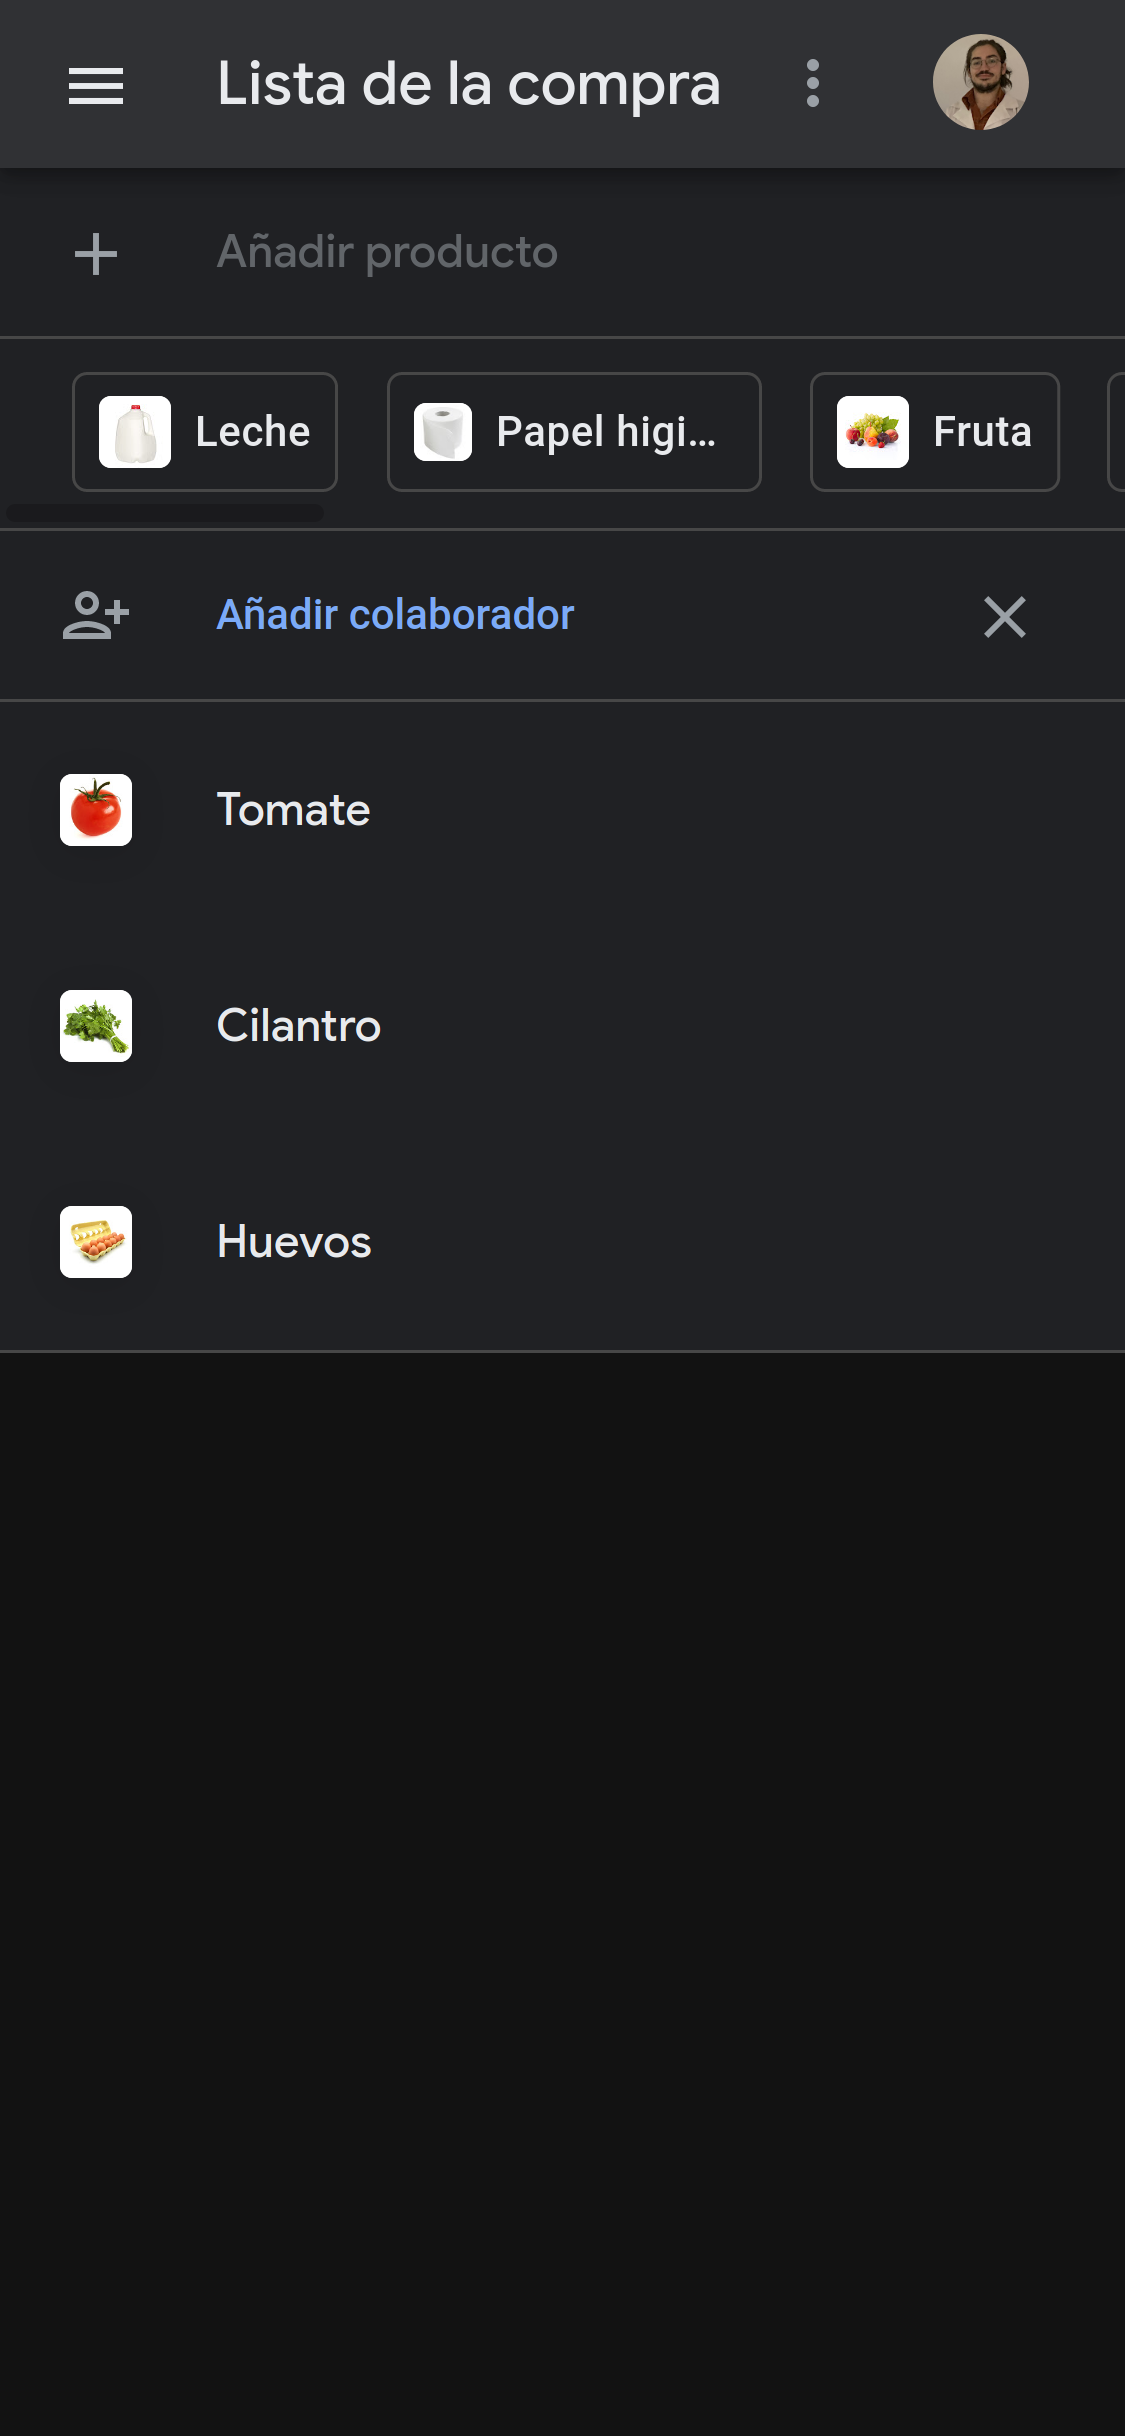
\includegraphics[trim=0 800 0 0, clip, width=.8\textwidth]{images/Screenshot_2020-11-09 Google Shopping List.png}
\end{minipage}
\section{Aplicaciones encontradas que son competencia parcial}
\section{Tablas de aplicaciones y funcionalidades}
\begin{tabular}{@{}rcccccccc@{}}
\textbf{Aplicación} & 
\rotatebox{90}{\textbf{Inventario}} &
\rotatebox{90}{\textbf{Crear listas}} &
\rotatebox{90}{\textbf{Compartir listas}} & 
\rotatebox{90}{\textbf{Notificaciones}} &
\rotatebox{90}{\textbf{Añadir fotos}} & 
\rotatebox{90}{\textbf{Añadir Precios}} &
\rotatebox{90}{\textbf{Categorías}} & 
\rotatebox{90}{\textbf{Voz}} \\
\toprule
Google Shopping List & \xmark & \cmark & \cmark & \xmark & \xmark & \xmark & \xmark & ? \\
\rowcolor{black!15}
Listonic             & \xmark & \cmark & \cmark & \cmark & \cmark & \cmark & \cmark & ? \\
\bottomrule
\end{tabular}

\begin{enumerate}
    \item Google Assistant
    \item Alexa
\end{enumerate}
\chapter{Lista de factoides}
\chapter{Conclusiones}
\section{Conclusión de conocer a los usuarios}
\section{Conclusión del análisis de la competencia}

El mercado de las listas de la compra parece ser muy amplio, pero el de gestión de despensa parece ser más reducido. Sólo hemos encontrado una aplicación con habilidades de comunicación (Out of Milk), que te permita decir que estás yendo a la compra o, pero no tiene gestión de productos y su caducidad.

Ninguna de las aplicaciones de gestión de despensa tenía un apartado muy desarrollado de consumo, para saber cuanto nos suele costar la compra, o gastos desglosados en el tiempo

Podemos observar que una funcionalidad con la que nuestros competidores no cuentan, es con la de poder escanear directamente el producto y no el código de barras, aunque sea técnicamente posible. (Google Lens, por ejemplo, es capaz de decirte el producto con una foto suya mediante búsqueda inversa de imágenes).

Ninguna aplicación cuenta tampoco con la habilidad de escanear el Ticket al completo y, mediante OCR\footnote{Reconocimiento Óptico de Caracteres (\textit{Optical Character Recognition})}, observar qué se ha comprado y añadirlo a la despensa, cosa que es capaz de hacer la aplicación de McDonnalds para comprobar tus productos consumidos y ofrecerte descuentos personalizados.
\appendix
\chapter{Modelo de consentimiento para la grabación}
\label{ch:consentimiento}
El \textbf{propósito} de este estudio es realizar una investigación para crear el producto \productname, para ello te realizaremos una entrevista corta que será grabada y guardada. Tu participación en este estudio es voluntaria, por lo que puedes decidir abandonar el estudio en cualquier momento sin razón aparente.

\subsubsection*{Consentimiento informado}
Yo, \underline{\hspace{7cm}}, he leído y entiendo el ámbito y naturaleza de este estudio y se me ha ofrecido la oportunidad de hacer preguntas. Entiendo que mi participación es voluntaria y tengo el derecho de retractarme sin alegar razones. Entiendo que se me proveerá de una copia de este documento. Acepto voluntariamente formar parte de este estudio.

\vspace{.5cm}
\begin{minipage}{.5\textwidth}
Firma del Participante:
\end{minipage}%
\begin{minipage}{.5\textwidth}
Firma del Investigador:
\end{minipage}

\vspace{3cm}

{\flushright En Madrid, a \underline{\hspace{10cm}}}

\chapter{Transcripción de las entrevistas}
\label{ch:entrevistas}
\section{Entrevista 1}
\begin{description}
    \preg ¿Cuál es su edad?
    \preg ¿Convive con más gente en su hogar? ¿Cuál es su relación con ellos?
    \preg ¿Tiene un smartphone o Tablet? ¿Es Android o iOS?
    \preg ¿Utiliza algún medio para anotar los productos que necesite comprar? ¿Cual?
    \preg Si no utiliza ningún medio, ¿Suele olvidarse de artículos que necesita comprar?
    \preg ¿Su móvil es de gama baja, media o alta?
    \preg ¿Con que frecuencia haces la compra? (diaria, semanal, mensual)
    \preg ¿Sueles comprar por internet? (Amazon Now, Carrefour Online, etc)
    \preg Si sueles comprar por internet, ¿Vas a recogerlo a tienda o pides envío?
    \preg Si vas a comprar al sitio, ¿Lo traes inmediatamente de vuelta (coche, en mano, transporte publico), o pides que te lo envíen?
    \preg ¿Pierdes mucho tiempo yendo a comprar, cuanto tiempo?
    \preg ¿Qué es lo que te hace perder el tiempo? ¿Buscar las cosas? ¿El transporte al sitio? ¿la caja?
    \preg ¿Sabes que es lo que tienes que comprar para la casa, o que es lo que hace falta? ¿Como lo recuerdas?
    \preg ¿Sabes que tipos de productos suele haber en tu casa con regularidad?
    \preg ¿Sabes en que lugares tienen los productos que necesitas?
    \preg ¿Sueles comprar mas económico, o por calidad del producto?
    \preg ¿Cuando vas a comprar, si no sabes con exactitud que producto escoger preguntas a alguien? (otros residentes de casa, trabajadores del super)
    \preg ¿Que partes del proceso de hacer la compra odias mas? ¿Cuales prefieres hacer? ¿Por qué? (comprar, organizar la compra, realizar el listado, etc.)
    \preg ¿Cuando vas a comprar usas alguna app para buscar información del producto que compras? (valores nutricionales, precio, valoraciones, etc). Si es así, ¿cuales utilizas?
    \preg ¿Sueles comprar cosas innecesarias?
    \preg ¿Suele tener mas de una lista de la compra? (Por ej. Lista de alimentos, lista de drogueria, etc) 
    \preg ¿Suele tener listas de la compra compartidas con diferentes grupos de personas? (por ej. lista de casa, lista para una fiesta, lista para cosas del trabajo, etc)
\end{description}    

\section{Entrevista 2}
\begin{description}
    \preg ¿Cuál es su edad?
    \preg ¿Convive con más gente en su hogar? ¿Cuál es su relación con ellos?
    \preg ¿Tiene un smartphone o Tablet? ¿Es Android o iOS?
    \preg ¿Utiliza algún medio para anotar los productos que necesite comprar? ¿Cual?
    \preg Si no utiliza ningún medio, ¿Suele olvidarse de artículos que necesita comprar?
    \preg ¿Su móvil es de gama baja, media o alta?
    \preg ¿Con que frecuencia haces la compra? (diaria, semanal, mensual)
    \preg ¿Sueles comprar por internet? (Amazon Now, Carrefour Online, etc)
    \preg Si sueles comprar por internet, ¿Vas a recogerlo a tienda o pides envío?
    \preg Si vas a comprar al sitio, ¿Lo traes inmediatamente de vuelta (coche, en mano, transporte publico), o pides que te lo envíen?
    \preg ¿Pierdes mucho tiempo yendo a comprar, cuanto tiempo?
    \preg ¿Qué es lo que te hace perder el tiempo? ¿Buscar las cosas? ¿El transporte al sitio? ¿la caja?
    \preg ¿Sabes que es lo que tienes que comprar para la casa, o que es lo que hace falta? ¿Como lo recuerdas?
    \preg ¿Sabes que tipos de productos suele haber en tu casa con regularidad?
    \preg ¿Sabes en que lugares tienen los productos que necesitas?
    \preg ¿Sueles comprar mas económico, o por calidad del producto?
    \preg ¿Cuando vas a comprar, si no sabes con exactitud que producto escoger preguntas a alguien? (otros residentes de casa, trabajadores del super)
    \preg ¿Que partes del proceso de hacer la compra odias mas? ¿Cuales prefieres hacer? ¿Por qué? (comprar, organizar la compra, realizar el listado, etc.)
    \preg ¿Cuando vas a comprar usas alguna app para buscar información del producto que compras? (valores nutricionales, precio, valoraciones, etc). Si es así, ¿cuales utilizas?
    \preg ¿Sueles comprar cosas innecesarias?
    \preg ¿Suele tener mas de una lista de la compra? (Por ej. Lista de alimentos, lista de drogueria, etc) 
    \preg ¿Suele tener listas de la compra compartidas con diferentes grupos de personas? (por ej. lista de casa, lista para una fiesta, lista para cosas del trabajo, etc)
\end{description}

\section{Entrevista 3 - Paloma}
\setresp{Paloma}
\begin{description}
    \preg ¿Cuál es su edad?
    \resp 24 años
    \preg ¿Convive con más gente en su hogar? ¿Cuál es su relación con ellos?
    \resp Vivo sola
    \preg ¿Tiene un smartphone o Tablet? ¿Es Android o iOS?
    \resp Tengo un smartphone Android.
    \preg ¿Utiliza algún medio para anotar los productos que necesite comprar? ¿Cual?
    \resp Utilizo el bloc de notas del móvil.
    \preg Si no utiliza ningún medio, ¿Suele olvidarse de artículos que necesita comprar?
    \resp Aun así se me suele olvidar muchos productos porque no los anoto en el bloc de notas.
    \preg ¿Su móvil es de gama baja, media o alta?
    \resp Gama media
    \preg ¿Con que frecuencia haces la compra? (diaria, semanal, mensual)
    \resp 2 veces por semana.
    \preg ¿Sueles comprar por internet? (Amazon Now, Carrefour Online, etc)
    \resp Nunca compro por internet, ya que prefiero escoger los alimentos que voy a consumir yo misma.
    \preg Si sueles comprar por internet, ¿Vas a recogerlo a tienda o pides envío?
    \resp 
    \preg Si vas a comprar al sitio, ¿Lo traes inmediatamente de vuelta (coche, en mano, transporte publico), o pides que te lo envíen?
    \resp Siempre inmediatamente y con la mano.
    \preg ¿Pierdes mucho tiempo yendo a comprar, cuanto tiempo?
    \resp Unos 30 minutos, vivo cerca del supermercado
    \preg ¿Qué es lo que te hace perder el tiempo? ¿Buscar las cosas? ¿El transporte al sitio? ¿la caja?
    \resp Sobre todo la caja, y en mirar productos que no tenía anotados.
    \preg ¿Sabes que es lo que tienes que comprar para la casa, o que es lo que hace falta? ¿Como lo recuerdas?
    \resp Intento siempre anotarlo todo y estar pendiente, aunque se me olvidan bastantes cosas.
    \preg ¿Sabes que tipos de productos suele haber en tu casa con regularidad?
    \resp Siempre suelo saberlo, soy bastante atenta para eso.
    \preg ¿Sabes en que lugares tienen los productos que necesitas?
    \resp Si, salvo que sea algo nuevo.
    \preg ¿Sueles comprar mas económico, o por calidad del producto?
    \resp Casi siempre busco la calidad del producto por encima del precio.
    \preg ¿Cuando vas a comprar, si no sabes con exactitud que producto escoger preguntas a alguien? (otros residentes de casa, trabajadores del super)
    \resp Pregunto a familiares que sé que entienden de esos productos.
    \preg ¿Que partes del proceso de hacer la compra odias mas? ¿Cuales prefieres hacer? ¿Por qué? (comprar, organizar la compra, realizar el listado, etc.)
    \resp Lo que mas odio es el pensar que tengo que ir, sobre todo en invierno cuando hace más frio. Lo que prefiero es el ver la nevera llena y saber que no tengo que volver hasta dentro de un par de días.
    Organizarlos no me preocupa demasiado.
    \preg ¿Cuando vas a comprar usas alguna app para buscar información del producto que compras? (valores nutricionales, precio, valoraciones, etc). Si es así, ¿cuales utilizas?
    \resp No utilizo ninguna app, ni nada por el estilo.
    \preg ¿Sueles comprar cosas innecesarias?
    \resp No suelo, aunque alguna vez lo he hecho.
    \preg ¿Suele tener mas de una lista de la compra? (Por ej. Lista de alimentos, lista de drogueria, etc) 
    \resp No.
    \preg ¿Suele tener listas de la compra compartidas con diferentes grupos de personas? (por ej. lista de casa, lista para una fiesta, lista para cosas del trabajo, etc)
    \resp Si es para alguna fiesta si, aunque con el covid ya no.
\end{description}

\section{Entrevista 4 - Emilio Sevilla}
\setresp{Emilio}
\begin{description}
    \preg ¿Cuál es su edad?
    \resp  Tengo 24 años
    \preg ¿Convive con más gente en su hogar? ¿Cuál es su relación con ellos?
    \resp  No, vivo sólo. 
    \preg ¿Tiene un smartphone o Tablet? ¿Es Android o iOS?
    \resp  Tengo un iphone.
    \preg ¿Utiliza algún medio para anotar los productos que necesite comprar? ¿Cual?
    \resp  Suelo apuntarlo en las notas del móvil
    \preg Si no utiliza ningún medio, ¿Suele olvidarse de artículos que necesita comprar?
    \resp  Pues como ya te he dicho si que utilizo un medio pero aun así se me suelen olvidar cosas.
    \preg ¿Su móvil es de gama baja, media o alta?
    \resp  Es de gama alta.
    \preg ¿Con que frecuencia haces la compra? (diaria, semanal, mensual)
    \resp  Depende pero por lo general semanalmente aunque como se me suele olvidar alguna cosa pues hay varios días que tengo que bajar a comprar.
    \preg ¿Sueles comprar por internet? (Amazon Now, Carrefour Online, etc)
    \resp  La compra nunca la hago por internet, pero para ropa por ejemplo si que lo hago, es decir, no me asustaría hacerlo.
    \preg Si sueles comprar por internet, ¿Vas a recogerlo a tienda o pides envío?
    \resp  Pues ya que lo compro por internet que me lo traigan a casa ¿no? si no me saltaría ese paso.
    \preg Si vas a comprar al sitio, ¿Lo traes inmediatamente de vuelta (coche, en mano, transporte publico), o pides que te lo envíen?
    \resp  Me lo llevo aunque pese mucho, si tengo que parar a descansar lo hago, eso nunca ha sido un problema para mi.
    \preg ¿Pierdes mucho tiempo yendo a comprar, cuanto tiempo?
    \resp  Pues un poco si, nunca organizo la lista de la compra en función a como están colocados los artículos en el super.
    \preg ¿Qué es lo que te hace perder el tiempo? ¿Buscar las cosas? ¿El transporte al sitio? ¿la caja?
    \resp  Como ya te he dicho pierdo tiempo en buscar las cosas. Si pudiera organizarlo por pasillos o algo así seguro que tardaría menos.
    \preg ¿Sabes que es lo que tienes que comprar para la casa, o que es lo que hace falta? ¿Como lo recuerdas?
    \resp  Pues por lo general durante la semana me voy dando cuenta de que necesito cosas e intento apuntarlo, pero siempre antes de ir a comprar abro la nevera, la despensa e intento pensar en qué me hace falta.
    \preg ¿Sabes que tipos de productos suele haber en tu casa con regularidad?
    \resp  Sí claro, los compro yo todos.
    \preg ¿Sabes en que lugares tienen los productos que necesitas?
    \resp  Si a no ser que sea algo nuevo o una marca específica que me han recomendado y no sé dónde la puedan vender cerca de mi casa.
    \preg ¿Sueles comprar mas económico, o por calidad del producto?
    \resp  Pues depende algunas cosas que uso más me interesa la calidad y otras que uso menos que sean baratas.
    \preg ¿Cuando vas a comprar, si no sabes con exactitud que producto escoger preguntas a alguien? (otros residentes de casa, trabajadores del super)
    \resp  Pues suelo preguntar al dependiente que productos son mejores y por qué. Pero a veces me gusta comprar uno, el próximo día que voy pruebo el otro y así decido cual comprar habitualmente.
    \preg ¿Que partes del proceso de hacer la compra odias mas? ¿Cuales prefieres hacer? ¿Por qué? (comprar, organizar la compra, realizar el listado, etc.)
    \resp  Pues claramente hacer cola y luego cargar hasta mi casa con ello. Prefiero la parte en la que me doy paseos por el super (risas).
    \preg ¿Cuando vas a comprar usas alguna app para buscar información del producto que compras? (valores nutricionales, precio, valoraciones, etc). Si es así, ¿cuales utilizas?
    \resp  Una vez me dijeron una app que escaneas el código de barras y te dice si el producto es bueno y eso. Pero nunca me la llegué a descargar.
    \preg ¿Sueles comprar cosas innecesarias?
    \resp  Alguna vez pero por lo general no.
    \preg ¿Suele tener mas de una lista de la compra? (Por ej. Lista de alimentos, lista de drogueria, etc) 
    \resp  Que va, todo junto de ahí los problemas (risas)
    \preg ¿Suele tener listas de la compra compartidas con diferentes grupos de personas? (por ej. lista de casa, lista para una fiesta, lista para cosas del trabajo, etc)
    \resp  Sí cuando nos vamos de barbacoa los amigos la hacemos por el grupo de whatsapp, pero siempre se olvidan cosas. Molaría tener una guardada por defecto para que no pasase eso.
\end{description}
\chapter{Encuesta mediante Google Forms} 
\label{ch:forms}
\section{Preguntas}
\section{Resultados}

\end{document}
